\chapter{Diagrammes de Penrose et formation d’un véritable trou noir}

Le diagramme de Kruskal décrit avec élégance le voisinage d’un horizon de Schwarzschild, mais un véritable trou noir n’est pas éternel : il se forme lors de l’effondrement de matière. Quelles parties du diagramme étendu subsistent après cette évolution physique ? Pour répondre, il nous faut un diagramme assez vaste pour contenir un espace-temps entier et assez rigoureux pour préserver le mouvement de la lumière. Nous commencerons par compactifier l’espace-temps plat, puis l’espace-temps de Schwarzschild, et enfin nous raccorderons les parties appropriées de part et d’autre d’une couche de rayonnement qui s’effondre.

\section{Au voisinage de l’horizon : rappel sur Kruskal et ses quatre quadrants}

Nous reprenons exactement là où le cours précédent s’est arrêté. Tout près de l’horizon de Schwarzschild, la géométrie ressemble localement à celle d’un espace plat. L’horizon lui-même se comporte comme le lieu d’une coordonnée polaire hyperbolique, un peu comme dans les coordonnées accélérées de l’espace-temps ordinaire de Minkowski. Dans cette représentation locale, nous imposons dès le départ une règle à laquelle nous ne dérogerons jamais : les rayons lumineux radiaux sont tracés à \(45^\circ\), et toute ligne d’univers de genre temps doit rester plus pentue que ces lignes de genre lumière.

Il vaut mieux considérer les coordonnées de ce rappel comme le temps et l’espace tels que les perçoit un observateur en chute libre. Dans ces coordonnées localement inertielles, le voisinage de l’horizon paraît presque plat. Mais un observateur qui tient à rester en suspension à rayon constant à l’extérieur du trou noir n’est pas inertiel. Dans le référentiel en chute libre, sa ligne d’univers est accélérée. Plus on se maintient près de l’horizon, plus l’accélération nécessaire pour y rester est grande. C’est ce que représentent physiquement les courbes extérieures dessinées sur la partie droite du tableau.

\begin{figure}[htbp]
\centering
\includegraphics[width=0.72\textwidth]{lecture_08_figure_02.png}
\caption{Schéma au tableau de la géométrie à quatre régions au voisinage de l’horizon. Les courbes rouges dans la région extérieure représentent une famille de lignes d’univers d’observateurs en suspension à rayon constant.}
\lectureframe{00:02:54}
\end{figure}

\begin{figure}[htbp]
\centering
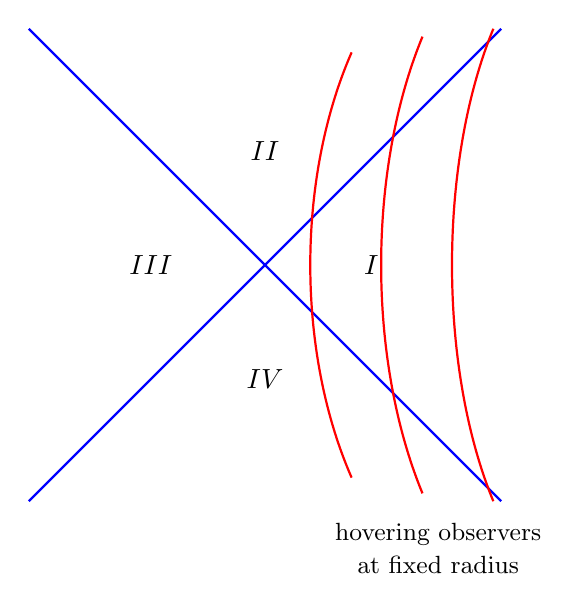
\begin{tikzpicture}[scale=1.0]
\draw[thick,blue] (-3,3) -- (3,-3);
\draw[thick,blue] (-3,-3) -- (3,3);

\draw[red,thick] (1.1,-2.7) .. controls (0.4,-1.1) and (0.4,1.1) .. (1.1,2.7);
\draw[red,thick] (2.0,-2.9) .. controls (1.3,-1.2) and (1.3,1.2) .. (2.0,2.9);
\draw[red,thick] (2.9,-3.0) .. controls (2.2,-1.3) and (2.2,1.3) .. (2.9,3.0);

\node at (1.35,0.0) {$I$};
\node at (0.0,1.45) {$II$};
\node at (-1.45,0.0) {$III$};
\node at (0.0,-1.45) {$IV$};

\node[align=center] at (2.2,-3.6) {\small hovering observers\\\small at fixed radius};
\end{tikzpicture}
\caption{Redessin net de la structure causale de type Kruskal utilisée dans le rappel. La région \(I\) est l’extérieur, la région \(II\) l’intérieur auquel nul ne peut échapper, et les régions \(III\) et \(IV\) appartiennent au prolongement formel que nous écarterons ensuite dans le cas d’un véritable trou noir issu d’un effondrement.}
\end{figure}

Cela suffit déjà à décrire ce que fait un trou noir. Dans la région extérieure \(I\), les objets et les signaux peuvent se diriger vers l’intérieur, mais ils peuvent aussi rester à l’extérieur ou repartir vers l’extérieur. Dans la région \(II\), en revanche, l’issue causale est fixée. Une fois à l’intérieur, aucune trajectoire causale orientée vers le futur ne permet de revenir à l’extérieur. Pour s’échapper de la région \(II\) et rejoindre l’une ou l’autre région extérieure, il faudrait qu’une trajectoire soit quelque part moins pentue que \(45^\circ\), et donc qu’elle dépasse la vitesse de la lumière. Toute trajectoire de genre temps admissible orientée vers le futur aboutit à la singularité.

Ce rappel introductif n’est pas une simple répétition. Il prépare le thème central du chapitre. Le diagramme de Kruskal est utile, mais il n’est pas entièrement pertinent physiquement pour un véritable trou noir.

\begin{classroomqa}
\audiencequestion{Quels sont les axes du diagramme, et quels observateurs à position fixe les courbes rouges représentent-elles ?}
\lecturerresponse{Les axes sont le temps et l’espace dans des coordonnées naturelles pour un observateur en chute libre. Au voisinage de l’horizon, cet observateur voit un espace-temps presque ordinaire et plat. Les courbes rouges à position constante correspondent, elles, à des observateurs maintenus immobiles à l’extérieur du trou noir. Leurs lignes d’univers sont accélérées, et l’accélération nécessaire augmente à mesure qu’ils s’approchent de l’horizon.
\lecturetimestamp{00:05:58--00:06:47}}
\end{classroomqa}

\section{Pourquoi compactifier ? D’un espace-temps infini à un tableau fini}

L’étape suivante relève de la méthode. Dans ces diagrammes, les directions de genre lumière s’étendent jusqu’à l’infini, tout comme le temps lui-même. Nous ne pouvons donc pas représenter l’espace-temps entier sur un tableau ordinaire sans changer de coordonnées. La motivation du professeur est très concrète : si nous voulons tout voir d’un seul coup et raisonner sur la structure causale globale, il nous faut un moyen de comprimer un espace-temps infini dans une région finie tout en gardant les rayons lumineux reconnaissables.

Il revient donc au cas simple, celui de l’espace-temps plat. Comme les problèmes qui nous intéressent sont à symétrie sphérique, nous supprimons les directions angulaires et ne gardons que le temps et la coordonnée radiale. Nous utilisons les coordonnées \(T\) et \(R\), avec
\[
R\ge 0,
\]
puisqu’une distance radiale négative n’a pas de sens en coordonnées polaires. Nous choisissons aussi des unités telles que
\[
c=1.
\]
Avec cette convention, le mouvement radial de la lumière est représenté par des lignes à \(45^\circ\).

Avant d’introduire l’application de compactification, le cours prend le temps de nous orienter dans le plan \(T\)-\(R\). On trace l’axe du temps, l’axe radial, quelques tranches à temps constant \(T=0,\pm1,\pm2\) et quelques lignes à rayon constant \(R=1,2,3\). Ce n’est pas du formalisme gratuit. Ces repères nous permettent de nous orienter et montrent clairement quelles caractéristiques nous voulons préserver lorsque le diagramme sera ensuite comprimé dans un espace fini.

Il y a aussi un point pédagogique subtil, mais important, concernant l’origine. Dans la représentation radiale réduite, un rayon lumineux dirigé exactement vers \(R=0\) semble rebondir sur l’origine et repartir vers l’extérieur. Mais rien ne se réfléchit physiquement sur une paroi. Dans la géométrie complète à symétrie sphérique, le rayon traverse simplement l’origine et ressort de l’autre côté. Ce rebond apparent vient uniquement du fait que nous travaillons dans le demi-plan \(R\ge 0\).

De même, un rayon lumineux qui manque l’origine semble d’abord suivre presque la même trajectoire, atteint son point de plus proche approche, puis repart vers l’extérieur. Dans ces coordonnées, on pourrait même croire que quelque chose l’a repoussé depuis l’origine. Mais là encore, il s’agit d’une description en coordonnées de la barrière familière associée au moment cinétique, et non d’une nouvelle force. Le professeur s’attarde sur ces exemples pour que le public puisse se fier au diagramme avant qu’il ne le déforme.

Voici maintenant l’étape essentielle. Nous allons comprimer et étirer le diagramme, tout en maintenant une chose : les rayons lumineux radiaux doivent rester des lignes à \(45^\circ\). C’est tout l’objectif de la compactification.

\begin{classroomqa}
\audiencequestion{L’origine choisie a-t-elle quelque chose de physiquement particulier, et les rayons qui semblent déviés témoignent-ils d’une force en ce point ?}
\lecturerresponse{Non. À ce stade, l’origine est simplement le centre choisi par les coordonnées sphériques. Le rebond et la déviation apparents viennent de la réduction du mouvement spatial complet à \(R\geq0\). La symétrie peut rendre un centre commode, comme dans le cas du Soleil, mais le choix des coordonnées n’y place ni trou noir ni paroi réfléchissante.
\lecturetimestamp{00:16:27--00:17:08}}
\end{classroomqa}

\section{L’espace-temps plat en coordonnées nulles et sous forme de Penrose}

Pour rendre la déformation précise, nous introduisons des coordonnées nulles. C’est la partie mathématiquement rigoureuse du cours, et le tableau rend cette étape explicite.

\begin{figure}[htbp]
\centering
\includegraphics[width=0.82\textwidth]{lecture_08_figure_03.png}
\caption{Le tableau \(T\)-\(R\) dégagé au moment de l’introduction de \(T^+=T+R\) et \(T^-=T-R\). L’origine radiale réduite est la ligne verticale bleue \(R=0\).}
\lectureframe{00:19:45}
\end{figure}

Nous définissons
\begin{align}
T^+ &= T+R, \\
T^- &= T-R.
\end{align}
Ces coordonnées sont adaptées au mouvement radial de la lumière. Un rayon lumineux radial entrant vérifie \(T^+=\text{const}\), tandis qu’un rayon lumineux radial sortant vérifie \(T^-=\text{const}\).

\paragraph{Démonstration détaillée.}
Dans ces coordonnées, la ligne \(R=0\) prend une forme particulièrement simple. En effet,
\begin{align}
R=0
&\iff T+R=T-R \\
&\iff T^+=T^-.
\end{align}
Ainsi, toute la frontière de genre temps \(R=0\) est décrite par la relation unique
\begin{equation}
R=0 \iff T^+=T^-.
\end{equation}

\begin{figure}[htbp]
\centering
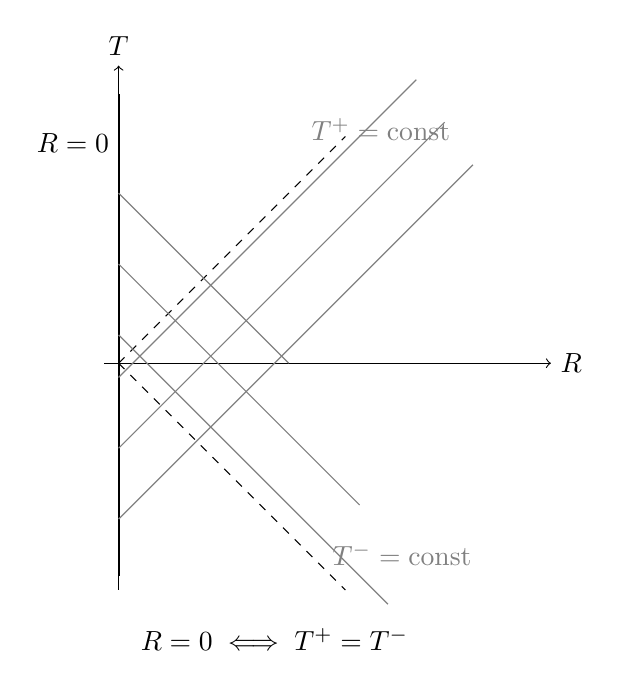
\begin{tikzpicture}[scale=0.9]
\draw[->] (-0.2,0) -- (6.1,0) node[right] {$R$};
\draw[->] (0,-3.2) -- (0,4.2) node[above] {$T$};

\draw[thick] (0,-3.0) -- (0,3.8);
\node[left] at (0,3.1) {$R=0$};

\draw[dashed] (0,0) -- (3.2,3.2);
\draw[dashed] (0,0) -- (3.2,-3.2);

\draw[gray] (0,2.4) -- (2.4,0);
\draw[gray] (0,1.4) -- (3.4,-2.0);
\draw[gray] (0,0.4) -- (3.8,-3.4);

\draw[gray] (0,-2.2) -- (5.0,2.8);
\draw[gray] (0,-1.2) -- (4.6,3.4);
\draw[gray] (0,-0.2) -- (4.2,4.0);

\node[gray] at (3.7,3.3) {$T^+=\mathrm{const}$};
\node[gray] at (4.0,-2.7) {$T^-=\mathrm{const}$};

\node at (2.2,-3.9) {$R=0 \iff T^+=T^-$};
\end{tikzpicture}
\caption{Redessin net dans le plan \(T\)-\(R\). Les deux familles de courbes nulles sont les lignes de niveau de \(T^+\) et \(T^-\), et la ligne \(R=0\) s’écrit aussi \(T^+=T^-\).}
\end{figure}

Nous passons maintenant à la compactification. Nous introduisons deux nouvelles coordonnées nulles \(U^\pm\), obtenues chacune à partir de la coordonnée \(T^\pm\) correspondante au moyen de la même fonction monotone bornée \(F\) :
\begin{align}
U^+ &= F(T^+), &
U^- &= F(T^-),
\end{align}
où
\begin{equation}
F(+\infty)=1,
\qquad
F(-\infty)=-1.
\end{equation}
Le choix commode retenu dans le cours est
\begin{equation}
F(x)=\tanh x,
\end{equation}
de sorte que
\begin{equation}
U^+ = \tanh(T^+),
\qquad
U^- = \tanh(T^-).
\end{equation}
La tangente hyperbolique n’a rien de sacré. C’est simplement une fonction régulière qui a le bon comportement aux limites et comprime ainsi des domaines de coordonnées infinis dans des domaines finis.

La structure nulle est préservée pour une raison simple. Si un rayon lumineux radial entrant vérifie \(T^+=\text{const}\), alors
\[
U^+=F(T^+)=\text{const},
\]
et, de même, si un rayon lumineux radial sortant vérifie \(T^-=\text{const}\), alors
\[
U^-=F(T^-)=\text{const}.
\]
La compactification ne fait donc que reparamétrer séparément les deux directions nulles, et les rayons lumineux radiaux restent des lignes à \(45^\circ\). La ligne de l’origine est transformée tout aussi simplement :
\[
T^+=T^- \Longrightarrow U^+=U^-.
\]

À ce stade, le demi-plan infini de l’espace-temps plat a été comprimé en un triangle fini. Le cours nous apprend ensuite à en lire les bords. L’infini spatial se réduit à un point unique \(i^0\). Les infinis de genre temps futur et passé sont \(i^+\) et \(i^-\). Les deux bords de genre lumière sont \(\mathcal{I}^+\) et \(\mathcal{I}^-\), souvent prononcés « scri-plus » et « scri-moins » ; c’est là que commencent et s’achèvent les rayons lumineux entrants et sortants.

\begin{figure}[htbp]
\centering
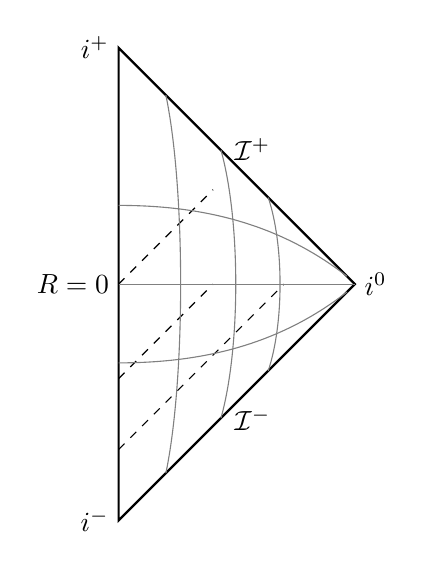
\begin{tikzpicture}[scale=1.0]
\draw[thick] (0,-3) -- (0,3) -- (3,0) -- cycle;

\node[left] at (0,3) {$i^+$};
\node[left] at (0,-3) {$i^-$};
\node[right] at (3,0) {$i^0$};
\node[left] at (0,0) {$R=0$};
\node[above right] at (1.35,1.45) {$\mathcal{I}^+$};
\node[below right] at (1.35,-1.45) {$\mathcal{I}^-$};

\draw[dashed] (0,-2.1) -- (2.1,0.0);
\draw[dashed] (0,-1.2) -- (1.2,0.0);
\draw[dashed] (0,0.0) -- (1.2,1.2);

\draw[gray] (0,0) -- (3,0);
\draw[gray] (0,1.0) .. controls (1.0,1.0) and (2.0,0.8) .. (2.9,0.1);
\draw[gray] (0,-1.0) .. controls (1.0,-1.0) and (2.0,-0.8) .. (2.9,-0.1);

\draw[gray] (0.6,-2.4) .. controls (0.85,-1.2) and (0.85,1.2) .. (0.6,2.4);
\draw[gray] (1.3,-1.7) .. controls (1.55,-0.8) and (1.55,0.8) .. (1.3,1.7);
\draw[gray] (1.9,-1.1) .. controls (2.1,-0.5) and (2.1,0.5) .. (1.9,1.1);
\end{tikzpicture}
\caption{Diagramme de Penrose de l’espace-temps plat à symétrie radiale réduite. Les courbes à temps constant s’étendent vers \(i^0\), tandis que les courbes à rayon constant partent de \(i^-\) et montent vers \(i^+\).}
\end{figure}

Gardons à l’esprit un dernier point du cours. Ces diagrammes ne préservent \emph{pas} les distances métriques. Ils préservent la structure causale. C’est cet invariant qui nous intéresse.

\begin{classroomqa}
\audiencequestion{Les lignes de temps constant dans le diagramme compactifié sont-elles censées être droites ?}
\lecturerresponse{Seule la tranche symétrique \(T=0\) est droite pour l’application choisie. Les autres courbes à \(T\) constant sont courbes, et leur forme précise dépend de la fonction de compactification. Les tranches correspondant aux temps très tardifs se resserrent toujours davantage contre le bord supérieur, bien que le temps ordinaire continue sans limite.
\lecturetimestamp{00:29:11--00:30:12}}
\end{classroomqa}

\section{La géométrie de Schwarzschild compactifiée}

Munis de la construction pour l’espace plat, nous revenons maintenant au trou noir et recommençons la même opération. Nous compactifions la géométrie de Kruskal en introduisant des coordonnées nulles et en comprimant leurs domaines infinis dans une figure finie. Le professeur décrit le résultat comme un rectangle diagonal ou un diagramme causal en forme de losange : l’horizon apparaît comme une frontière nulle, les lignes d’univers des observateurs en suspension à l’extérieur restent en dehors, et la région intérieure aboutit à une singularité désormais visible sur la page.

Le point physique crucial est que la singularité n’est \emph{pas} à l’infini pour l’observateur en chute libre. Après avoir franchi l’horizon, il lui reste un temps propre fini avant de heurter la singularité. Le diagramme de Penrose le rend visuellement incontournable.

L’horizon est de nouveau repéré par la condition de Schwarzschild
\begin{equation}
1-\frac{2MG}{r}=0
\qquad \Longleftrightarrow \qquad
r=2MG.
\end{equation}
L’égalité \(r=2MG\) marque le rayon auquel le facteur de Schwarzschild change de signe.

\begin{figure}[htbp]
\centering
\includegraphics[width=0.72\textwidth]{lecture_08_figure_04.png}
\caption{Schéma au tableau opposant le diagramme étendu formel à la région du trou noir qui a une pertinence physique. L’inscription rouge \emph{singularité} est clairement indiquée au tableau.}
\lectureframe{00:37:59}
\end{figure}

\begin{figure}[htbp]
\centering
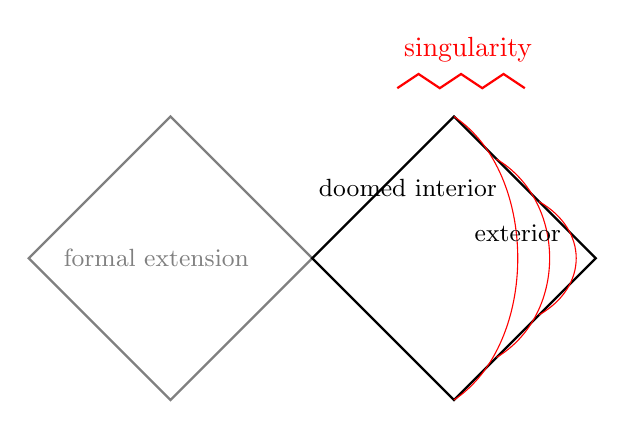
\begin{tikzpicture}[scale=0.9]
\draw[gray,thick] (-4,0) -- (-2,2) -- (0,0) -- (-2,-2) -- cycle;
\draw[thick] (0,0) -- (2,2) -- (4,0) -- (2,-2) -- cycle;

\draw[red,thick] (1.2,2.4) -- (1.5,2.6) -- (1.8,2.4) -- (2.1,2.6) -- (2.4,2.4) -- (2.7,2.6) -- (3.0,2.4);
\node[red] at (2.2,2.95) {singularity};

\draw[red] (2.0,-2.0) .. controls (3.2,-1.2) and (3.2,1.2) .. (2.0,2.0);
\draw[red] (2.6,-1.4) .. controls (3.6,-0.8) and (3.6,0.8) .. (2.6,1.4);
\draw[red] (3.2,-0.8) .. controls (3.9,-0.4) and (3.9,0.4) .. (3.2,0.8);

\node at (2.9,0.35) {\small exterior};
\node at (1.35,1.0) {\small doomed interior};
\node[gray] at (-2.2,0.0) {\small formal extension};
\end{tikzpicture}
\caption{Redessin prudent de la structure causale mise en avant dans le cours : l’extérieur qui subsiste, l’intérieur condamné, la singularité future et le contraste avec la partie supplémentaire, formelle, du prolongement.}
\end{figure}

Le cours est très direct sur ce point. Si vous êtes dans la région extérieure, vous pouvez encore vous échapper ou tomber à l’intérieur. Si vous êtes dans la région intérieure, vous êtes condamné. Le diagramme dit déjà tout ce qui importe sur le mouvement causal orienté vers le futur.

Les quadrants \(III\) et \(IV\) sont des parties légitimes de la solution de Kruskal maximalement prolongée. La région \(III\) fournit un second extérieur, et la région \(IV\) est la région du trou noir renversée dans le temps. Elles ne font toutefois pas partie de l’espace-temps d’un trou noir ordinaire formé par effondrement. La solution prolongée est instructive mathématiquement précisément parce que la construction par effondrement nous montrera quelles parties doivent être écartées.

\section{Tranches spatiales, sphères, et pont d’Einstein--Rosen}

Considérons maintenant une tranche spatiale du diagramme compactifié et demandons-nous à quoi elle ressemble en tant qu’\emph{espace} plutôt qu’en tant qu’espace-temps. C’est ici qu’intervient l’image du trou de ver, et qu’il faut éviter de laisser la représentation spatiale devancer le raisonnement causal.

Comme les directions angulaires ont été supprimées, chaque point du diagramme radial représente une sphère. Au rayon de Schwarzschild \(r\), son aire vaut
\begin{equation}
A=4\pi r^2.
\end{equation}
Une tranche spatiale est donc une famille de sphères, et non une simple courbe unidimensionnelle. Leur taille varie lorsqu’on se déplace le long de la tranche.

Loin du trou noir, les sphères sont très grandes. En se déplaçant vers l’intérieur, leur rayon diminue jusqu’à atteindre un minimum à l’horizon,
\begin{equation}
r_{\min}=2MG.
\end{equation}
Si l’on poursuit à travers le prolongement formel, les sphères se dilatent de nouveau en direction d’une autre région asymptotique. C’est l’image du pont d’Einstein--Rosen.

\begin{figure}[htbp]
\centering
\includegraphics[width=0.72\textwidth]{lecture_08_figure_05.png}
\caption{Diagramme de Kruskal étendu avec la tranche spatiale verte utilisée pour construire la géométrie du pont. Chaque point de cette tranche représente une sphère ; son rayon minimal est indiqué par \(r=2MG\).}
\lectureframe{00:41:30}
\end{figure}

Le tableau ne montre qu’une partie du facteur de Schwarzschild pertinent,
\begin{equation}
1-\frac{2MG}{r},
\end{equation}
et le col se trouve au même rayon particulier \(r=2MG\).

\begin{figure}[htbp]
\centering
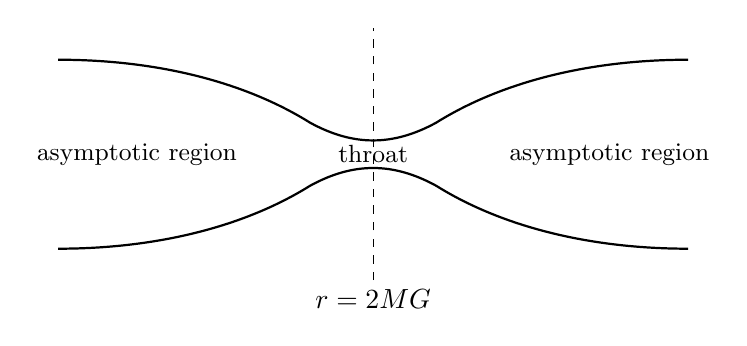
\begin{tikzpicture}[scale=1.0]
\draw[thick] (-4,1.2)
.. controls (-2.7,1.2) and (-1.6,0.9) .. (-0.8,0.4)
.. controls (-0.25,0.1) and (0.25,0.1) .. (0.8,0.4)
.. controls (1.6,0.9) and (2.7,1.2) .. (4,1.2);

\draw[thick] (-4,-1.2)
.. controls (-2.7,-1.2) and (-1.6,-0.9) .. (-0.8,-0.4)
.. controls (-0.25,-0.1) and (0.25,-0.1) .. (0.8,-0.4)
.. controls (1.6,-0.9) and (2.7,-1.2) .. (4,-1.2);

\draw[dashed] (0,-1.6) -- (0,1.6);
\node[below] at (0,-1.6) {$r=2MG$};
\node at (0,0) {\small throat};
\node at (-3.0,0) {\small asymptotic region};
\node at (3.0,0) {\small asymptotic region};
\end{tikzpicture}
\caption{Schéma d’une tranche spatiale à travers la géométrie de Schwarzschild étendue. Il s’agit d’une reconstruction prudente de l’image du pont présentée dans le cours, et non d’un calcul littéral d’immersion.}
\end{figure}

Vient maintenant la correction. La tranche suggère un pont entre deux régions asymptotiques, ce qui invite à penser que l’on pourrait passer d’un univers à l’autre en traversant le col. Le cours laisse d’abord cette idée émerger, puis l’écarte par un argument causal. Pour aller d’une région extérieure à l’autre, une ligne d’univers devrait quelque part être moins pentue qu’une ligne nulle à \(45^\circ\) sur le diagramme de Penrose. C’est interdit. Le pont d’Einstein--Rosen n’est donc pas traversable.

Le professeur souligne aussi pourquoi la représentation spatiale peut induire en erreur. Elle représente l’\emph{espace à un instant donné} ; or le temps causal disponible ne suffit tout simplement pas pour le traverser. On pourrait dire, en termes imagés, que le pont s’ouvre et se referme avant que quoi que ce soit ait pu le franchir. Mieux encore, il suffit de revenir au diagramme de Penrose et d’y lire la réponse causale.

\section{Construire un véritable trou noir à partir d’une couche nulle entrante}

À ce stade, le cours change complètement de problème. Nous ne cherchons plus à déduire les propriétés d’un trou noir éternel. Nous en construisons un véritable.

Le modèle est choisi pour sa simplicité. Nous imaginons non pas une étoile qui s’effondre avec une structure interne complexe, mais une mince couche sphérique de rayonnement entrant. C’est une couche de lumière, qui se déplace donc vers l’intérieur à la vitesse de la lumière. À un rayon suffisamment petit, l’énergie de cette couche est assez concentrée pour qu’un trou noir se forme.

Le second ingrédient est le théorème des coquilles sous sa forme relativiste générale.

\paragraph{Remarque.} Pour la couche sphérique à symétrie sphérique utilisée dans ce cours, la région intérieure est un espace-temps plat, tandis que la région extérieure est décrite par la géométrie de Schwarzschild. C’est la règle pratique du théorème des coquilles, ou l’énoncé de type Birkhoff, utilisé dans le cours. Elle n’est pas démontrée ici.

Le professeur motive cet énoncé en rappelant d’abord le théorème des coquilles newtonien : à l’intérieur d’une coquille sphérique, le champ gravitationnel est nul, tandis qu’à l’extérieur il est identique à celui d’une masse ponctuelle placée au centre. Il énonce ensuite la version relativiste correspondante, dans la seule forme nécessaire ici : l’intérieur est plat, l’extérieur est décrit par la géométrie de Schwarzschild. La coquille peut se déplacer ; la règle reste la même.

Cela suffit pour construire l’espace-temps de l’effondrement. La coquille elle-même est nulle, elle doit donc être tracée à \(45^\circ\). D’un côté de cette ligne nulle, la géométrie est plate. De l’autre, elle est décrite par la géométrie de Schwarzschild. On peut résumer la règle ainsi :
\begin{equation}
\begin{aligned}
\text{inside shell} &= \text{flat spacetime},\\
\text{outside shell} &= \text{Schwarzschild geometry}.
\end{aligned}
\end{equation}

La prescription de raccordement devient alors presque embarrassante de simplicité :

\begin{enumerate}
\item Tracer le diagramme de Penrose plat et ne garder que la région située à l’intérieur de la couche entrante.
\item Tracer le diagramme de Penrose de Schwarzschild et ne garder que la région située à l’extérieur de cette même couche.
\item Écarter les mauvaises parties.
\item Raccorder les deux parties conservées le long de la trajectoire de la couche.
\end{enumerate}

C’est exactement ainsi que le professeur procède au tableau : il écarte la mauvaise moitié d’un diagramme, puis la mauvaise moitié de l’autre, et raccorde les bonnes moitiés le long de la couche.

\begin{figure}[htbp]
\centering
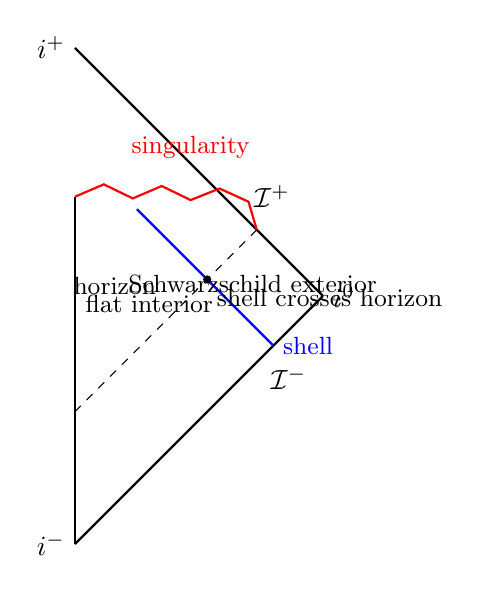
\begin{tikzpicture}[scale=1.05]
\coordinate (im) at (0,-3.0);
\coordinate (ip) at (0,3.0);
\coordinate (i0) at (3.0,0.0);
\coordinate (S)  at (0,1.2);
\coordinate (E)  at (2.2,0.8);
\coordinate (P)  at (2.4,-0.6);
\coordinate (Q)  at (0.75,1.05);
\coordinate (H)  at (0,-1.4);
\coordinate (X)  at (1.6,0.2);

\draw[thick] (im) -- (S);
\draw[thick] (im) -- (i0);
\draw[thick] (ip) -- (i0);

\draw[red,thick] (S) -- (0.35,1.35) -- (0.7,1.18) -- (1.05,1.33) -- (1.4,1.16) -- (1.75,1.30) -- (2.1,1.14) -- (E);
\node[red,above] at (1.4,1.55) {\small singularity};

\draw[thick,blue] (P) -- (Q);
\node[blue,right] at (P) {\small shell};

\draw[dashed] (H) -- (E);
\node[above left] at (1.1,-0.1) {\small horizon};

\filldraw (X) circle (1.2pt);
\node[below right] at (X) {\small shell crosses horizon};

\node at (0.9,-0.1) {\small flat interior};
\node at (2.15,0.15) {\small Schwarzschild exterior};

\node[left] at (im) {$i^-$};
\node[left] at (ip) {$i^+$};
\node[right] at (i0) {$i^0$};
\node[below right] at (2.25,-0.75) {$\mathcal{I}^-$};
\node[above right] at (2.05,0.95) {$\mathcal{I}^+$};
\end{tikzpicture}
\caption{Reconstruction causale de la géométrie de l’effondrement. La couche est une ligne nulle entrante ; l’espace-temps plat est conservé du côté intérieur et la géométrie de Schwarzschild du côté extérieur.}
\end{figure}

\begin{figure}[htbp]
\centering
\includegraphics[width=0.76\textwidth]{lecture_08_figure_06.png}
\caption{Construction finale au tableau, après raccordement de la région intérieure plate et de la région extérieure de Schwarzschild le long de la couche bleue en chute. La ligne pointillée \(45^\circ\) est tracée vers le passé à partir de l’extrémité future de la singularité pour repérer l’horizon des événements.}
\lectureframe{00:57:30}
\end{figure}

La couche elle-même ne subit rien de particulier au moment où elle passe simplement de la partie plate du diagramme à la partie de Schwarzschild. C’est une couche de genre lumière, qui poursuit sa chute vers l’intérieur jusqu’à atteindre la singularité. La structure essentielle ne tient pas à un phénomène local spectaculaire sur la couche ; elle tient à l’organisation causale de l’espace-temps raccordé.

\begin{classroomqa}
\audiencequestion{Y a-t-il une discontinuité lorsque la couche qui s’effondre franchit son rayon de Schwarzschild ?}
\lecturerresponse{Non. Rien de singulier ne se produit localement lors de ce franchissement. La couche poursuit sa trajectoire nulle. L’événement particulier est de nature causale : après que la couche a franchi son propre rayon \(2MG\), aucune trajectoire orientée vers le futur ne peut la ramener à l’infini.
\lecturetimestamp{00:56:19--00:56:42}}
\end{classroomqa}

\section{L’horizon avant l’arrivée : l’énigme de l’horizon des événements}

Voici le point culminant conceptuel du cours. Une fois l’espace-temps de l’effondrement construit, la question naturelle est : où se trouve l’horizon ? Ou, pour reprendre les mots du professeur, où est le point de non-retour ?

\paragraph{Définition.} L’horizon des événements est la frontière entre les événements qui peuvent encore envoyer un signal causal orienté vers le futur jusqu’à \(\mathcal{I}^+\) et ceux qui ne le peuvent pas.

Le cours le repère sur le diagramme. Partons du coin où la singularité rejoint l’infini nul futur et traçons vers le passé une ligne nulle à \(45^\circ\). Cette ligne nulle tracée vers le passé est l’horizon des événements.

Le professeur insiste ensuite sur un second point, celui qui met les étudiants mal à l’aise. L’horizon n’apparaît pas simplement au moment où la couche franchit son propre rayon de Schwarzschild pour ensuite rester en place. Dans le dessin agrandi au tableau, l’horizon commence par former une minuscule région piégée près du centre, s’étend vers l’extérieur à travers une partie de l’espace-temps encore plate, puis ne rejoint que plus tard la couche entrante. À cet événement de rencontre, la couche franchit son propre rayon de Schwarzschild. Au-dessus de cet événement, l’horizon est l’horizon ordinaire à rayon constant du trou noir formé.

\begin{figure}[htbp]
\centering
\resizebox{0.96\linewidth}{!}{%
\begin{tikzpicture}[scale=1.08,>=Latex]
\coordinate (im) at (0,-3.0);
\coordinate (ip) at (0,3.0);
\coordinate (i0) at (3.0,0.0);
\coordinate (S)  at (0,1.2);
\coordinate (E)  at (2.2,0.8);
\coordinate (P)  at (2.4,-0.6);
\coordinate (Q)  at (0.75,1.05);
\coordinate (H)  at (0,-1.4);
\coordinate (X)  at (1.6,0.2);

\draw[thick] (im) -- (S);
\draw[thick] (im) -- (i0);
\draw[thick] (ip) -- (i0);

\draw[red,thick] (S) -- (0.35,1.35) -- (0.7,1.18) -- (1.05,1.33) -- (1.4,1.16) -- (1.75,1.30) -- (2.1,1.14) -- (E);
\node[red,above left] at (S) {\small singularity};

\draw[very thick,red] (H) -- (E);

\draw[thick,blue] (P) -- (Q);

\filldraw (X) circle (1.2pt);

\draw[gray] (0.0,-2.1) .. controls (0.85,-1.95) and (1.9,-1.3) .. (2.8,-0.2);
\draw[gray] (0.0,-1.2) .. controls (0.95,-1.0) and (1.8,-0.45) .. (2.45,0.35);
\draw[gray] (0.0,-0.2) .. controls (0.8,-0.05) and (1.45,0.35) .. (1.95,0.95);

\node[below right] at (2.28,-0.72) {$\mathcal{I}^-$};
\node[above right] at (2.12,0.92) {$\mathcal{I}^+$};

\draw[very thick,red] (3.2,-1.15) -- (3.75,-1.15);
\node[anchor=west] at (3.85,-1.15) {\small event horizon};
\draw[thick,blue] (3.2,-1.55) -- (3.75,-1.55);
\node[anchor=west] at (3.85,-1.55) {\small infalling shell};
\filldraw (3.48,-1.95) circle (1.2pt);
\node[anchor=west] at (3.85,-1.95)
  {\small shell reaches \(r=2MG\)};
\end{tikzpicture}
}
\caption{Diagramme de l’effondrement où l’horizon des événements tracé vers le passé est mis en évidence. Une partie de l’horizon se trouve dans une région encore localement plate, que la couche n’a pas encore atteinte.}
\end{figure}

C’est cet effet frappant que le reste du cours examine en détail. Une partie de l’horizon se trouve dans l’espace-temps plat. La couche n’y est pas encore arrivée, et elle n’est même pas visible sur le cône de lumière passé de l’observateur. L’observateur ne ressent aucun champ gravitationnel et ne peut pourtant pas s’échapper. La raison n’est pas une force locale. Elle tient à l’avenir causal global de l’événement.

\begin{classroomqa}
\audiencequestion{La construction signifie-t-elle qu’on ne peut pas franchir la couche, ou qu’on ne peut pas franchir l’horizon ? Où se trouve la couche lorsque son horizon est encore à l’intérieur de celle-ci ?}
\lecturerresponse{On peut franchir la couche. L’horizon est une autre surface nulle : c’est la frontière entre les événements qui peuvent communiquer avec \(\mathcal I^+\) et ceux qui ne le peuvent pas. La couche entrante rejoint cette frontière précisément lorsqu’elle franchit le rayon de Schwarzschild associé à son énergie totale. Avant cette rencontre, une partie de l’horizon des événements traverse l’intérieur plat ; après, la couche se trouve à l’intérieur du trou noir formé.
\lecturetimestamp{00:58:42--01:01:06}}
\end{classroomqa}

\begin{classroomqa}
\audiencequestion{Si l’intérieur est plat et que l’enveloppe est encore loin, pourquoi quelqu’un situé juste à l’intérieur de l’horizon ne peut-il pas traverser l’enveloppe à pied avant qu’elle ne l’atteigne ?}
\lecturerresponse{Tracez la ligne d’univers dirigée vers l’extérieur la plus rapide, celle d’un rayon lumineux à \(45^\circ\). Depuis un événement situé à l’intérieur de l’horizon obtenu par prolongement vers le passé, même ce rayon rencontre l’enveloppe entrante trop tard et finit à la singularité. À pied, le trajet est encore plus lent. L’expression \emph{l’enveloppe n’a pas encore franchi l’horizon} est incomplète tant qu’on n’a pas choisi de coordonnée temporelle ; le diagramme causal fournit la réponse indépendante des coordonnées. Le fond diffus cosmologique entrant n’est pas le même exemple, car ce n’est pas une enveloppe sphérique en effondrement qui crée cette géométrie.
\lecturetimestamp{01:01:07--01:04:03}}
\end{classroomqa}

\section{Miroirs et tentatives de modifier l’avenir}

Les questions transforment maintenant le diagramme en laboratoire. Supposons qu’une couche lumineuse entrante puisse être réfléchie avant d’être piégée. L’histoire de l’effondrement supposée changerait alors, et l’horizon des événements aussi. Il n’y a là aucune contradiction : l’horizon des événements n’est défini qu’une fois spécifiée l’histoire complète de l’espace-temps.

\begin{classroomqa}
\audiencequestion{Que se passerait-il si l’on plaçait un miroir parfaitement réfléchissant juste à l’extérieur du rayon de Schwarzschild qui allait se former, de sorte que la couche rebondisse vers l’extérieur ?}
\lecturerresponse{Dans cette histoire idéalisée, la ligne nulle entrante s’inverse au niveau du miroir, repart vers l’extérieur et atteint la frontière future ; le trou noir du diagramme initial ne se forme pas. Un miroir véritablement dépourvu de masse est impossible, et un miroir physique apporte sa propre énergie-impulsion, mais cette expérience de pensée fait ressortir le point logique : l’évasion n’est impossible qu’après que la couche a franchi l’horizon des événements réel.
\lecturetimestamp{01:04:33--01:05:54}}
\end{classroomqa}

\begin{classroomqa}
\audiencequestion{Un observateur qui sait que l’enveloppe arrive pourrait-il envoyer rapidement un miroir ou un signal pour la faire rebrousser chemin ?}
\lecturerresponse{Seulement si l’appareil nécessaire peut être placé assez tôt à l’extérieur de l’horizon. Alice peut convenir à l’avance avec Bob qu’il envoie l’enveloppe et savoir ainsi ce qui se prépare avant de la voir. Cependant, une fois son événement situé à l’intérieur de l’horizon, ni un miroir ni une instruction ne peuvent atteindre à temps le point extérieur requis. Savoir à l’avance ce qui va se passer dans l’expérience ne crée pas de chemin causal que le diagramme interdit.
\lecturetimestamp{01:05:55--01:08:18}}
\end{classroomqa}

\begin{classroomqa}
\audiencequestion{Qu’advient-il d’un miroir déjà à l’intérieur de l’horizon, et la singularité se trouve-t-elle à une distance infinie dans son avenir ?}
\lecturerresponse{Le miroir n’est qu’un autre objet condamné. Il peut réfléchir la lumière localement, mais la lumière réfléchie, le miroir et Alice finissent tous à la singularité. Une ligne d’univers générique en chute atteint celle-ci en un temps propre fini. Seul le sommet idéal du diagramme compactifié se trouve à une distance infinie. Tenter de rester près de ce sommet exigerait une accélération et une énergie non bornées ; en outre, entre deux événements fixés, une horloge accélérée accumule moins de temps propre qu’une horloge inertielle, et non davantage.
\lecturetimestamp{01:08:19--01:10:19}}
\end{classroomqa}

\begin{classroomqa}
\audiencequestion{Si l’enveloppe en effondrement est énorme, quelqu’un qui se trouve à l’intérieur de l’enveloppe, mais loin de son futur centre, peut-il simplement rester sur place pendant qu’elle passe ?}
\lecturerresponse{Oui, à condition que l’événement de cette personne se situe encore à l’extérieur de l’horizon des événements. Se trouver à l’intérieur de l’enveloppe matérielle n’est pas la même chose que se trouver à l’intérieur du trou noir. Le rayonnement peut frapper l’observateur et le blesser, mais il s’agit d’une interaction locale avec l’enveloppe, distincte de la question causale de la possibilité de s’échapper.
\lecturetimestamp{01:10:21--01:11:24}}
\end{classroomqa}

\section{Tranches temporelles et croissance de l’horizon}

Un \emph{instant de temps} en espace-temps courbe désigne une hypersurface de genre espace choisie. Une famille de telles surfaces forme un feuilletage, et attribuer un nombre à chaque surface définit une coordonnée temporelle. Des feuilletages différents découpent différemment le même diagramme d’effondrement. Ils ne s’accordent pas sur les événements distants qui sont simultanés, mais ne modifient pas les rayons lumineux nuls qui atteignent l’infini.

\begin{figure}[htbp]
\centering
\includegraphics[width=0.77\textwidth]{lecture_08_figure_07.png}
\caption{Le diagramme tardif au tableau, avec plusieurs tranches vertes de genre espace. Ces tranches définissent une coordonnée temporelle ; les frontières nulles noires et leurs relations causales sont indépendantes de ce choix.}
\lectureframe{01:17:30}
\end{figure}

\begin{classroomqa}
\audiencequestion{Peut-on reformuler le problème en comparant, à un instant donné, la distance entre l’observateur et l’horizon à celle entre l’horizon et la coquille ?}
\lecturerresponse{Cela peut donner une intuition utile une fois qu’un feuilletage a été choisi, mais l’expression \emph{à un instant donné} dépend des coordonnées. La construction rigoureuse consiste à tracer une famille de tranches de genre espace. Les premières rencontrent une coquille de grand rayon, sans région centrale piégée ; les suivantes rencontrent l’horizon qui s’agrandit, à l’intérieur de la coquille qui continue à tomber ; une tranche particulière passe par l’événement où la coquille franchit son propre rayon de Schwarzschild.
\lecturetimestamp{01:11:26--01:14:21}}
\end{classroomqa}

\begin{classroomqa}
\audiencequestion{Le rayon de Schwarzschild augmente-t-il à mesure que l’horizon s’étend vers l’extérieur, et pourquoi l’horizon continue-t-il de grandir après que la coquille l’a franchi ?}
\lecturerresponse{Le rayon de Schwarzschild final \(2MG\) est fixé, puisque la masse totale \(M\) est fixée. Ce qui augmente sur les premières tranches de genre espace, c’est le rayon aréolaire de la section de l’horizon. Il part du centre, augmente jusqu’à rencontrer la coquille à \(r=2MG\), puis cesse d’augmenter. Au-dessus de l’événement de rencontre, l’horizon suit la ligne \(r\) = constante, soit \(r=2MG\), même si la compactification ne donne pas à cette ligne une apparence verticale ni une métrique uniforme.
\lecturetimestamp{01:14:22--01:16:15}}
\end{classroomqa}

\begin{classroomqa}
\audiencequestion{Qu’arrive-t-il à un observateur initialement situé à la moitié du rayon de Schwarzschild final ? Cet observateur ne devrait-il pas ne ressentir la gravité qu’à l’arrivée de la coquille ?}
\lecturerresponse{Exactement. L’observateur franchit d’abord l’horizon des événements qui s’agrandit alors qu’il se trouve encore dans l’espace-temps plat, et ne ressent aucune force soudaine. La coquille de rayonnement qui tombe est matérielle et pourra être ressentie plus tard ; l’horizon des événements, lui, ne l’est pas. Le franchir signifie seulement que toute trajectoire causale future échoue désormais à atteindre l’infini. En ce sens précis, l’horizon est fantomatique.
\lecturetimestamp{01:16:17--01:17:45}}
\end{classroomqa}

\begin{classroomqa}
\audiencequestion{Un observateur qui commence assez tôt peut-il se déplacer vers l’extérieur plus vite que l’horizon ne s’agrandit et s’échapper ?}
\lecturerresponse{Les événements situés à l’extérieur de l’horizon ont des trajectoires causales sortantes vers \(\mathcal I^+\) ; ceux qui sont à l’intérieur n’en ont pas. Sur une tranche choisie, on peut comparer la distance radiale disponible au temps qui reste avant que la coquille entrante ne ferme la voie, mais les lignes nulles donnent le critère exact. Aucun observateur ne voit un horizon matériel se précipiter vers l’extérieur, car il n’existe aucune surface locale à voir.
\lecturetimestamp{01:17:46--01:18:54}}
\end{classroomqa}

\section{Ce que le diagramme préserve}

Les formes sur la page ne doivent pas être interprétées comme un dessin à l’échelle. Un petit coin peut représenter une région infinie de l’espace-temps, tandis qu’une grande zone peut correspondre à un intervalle physique modeste. La compactification sacrifie délibérément les dimensions métriques pour préserver les directions nulles. Ce qui est conservé, c’est la causalité : qui peut envoyer un signal à qui, quels événements peuvent en influencer d’autres, et quelles lignes d’univers sont piégées par la limite imposée par la vitesse de la lumière.

\begin{classroomqa}
\audiencequestion{Si l’image déforme à ce point les longueurs et les durées, que représente-t-elle fidèlement ?}
\lecturerresponse{Elle représente les rayons lumineux et, par conséquent, la structure causale. Pour localiser l’horizon des événements, il faut suivre à rebours le dernier rayon lumineux nul sortant depuis l’infini futur. Essayer de déduire la réponse des distances apparentes sur la page n’est pas fiable. Une fois le diagramme causal tracé, les questions portant sur les signaux, l’évasion et l’impossibilité du retour trouvent une réponse géométrique, même si l’échelle métrique a été supprimée.
\lecturetimestamp{01:18:56--01:21:45}}
\end{classroomqa}

\begin{classroomqa}
\audiencequestion{Combien de temps faut-il pour être suffisamment à l’aise avec les diagrammes de Penrose pour les utiliser de manière intuitive ?}
\lecturerresponse{Peu de temps. La méthode pratique consiste à les tracer, à suivre les lignes nulles et à tester différentes lignes d’univers possibles jusqu’à ce que les contraintes causales deviennent familières. Ici, l’intuition s’acquiert en travaillant avec les diagrammes, et non en faisant des suppositions sans eux.
\lecturetimestamp{01:21:49--01:22:05}}
\end{classroomqa}

\begin{classroomqa}
\audiencequestion{Cette méthode visuelle est-elle à l’opposé de la mécanique quantique, où les mathématiques sont souvent plus fiables qu’une représentation visuelle ?}
\lecturerresponse{Dans une large mesure, oui. La relativité générale est une théorie classique. Il est difficile de se représenter littéralement un espace-temps courbe à quatre dimensions, et un diagramme de Penrose reste abstrait, mais sa géométrie causale peut être tracée et explorée bien plus avant que la réalité sous-jacente de la mécanique quantique. C’est en partie ce qui rend ces diagrammes si puissants.
\lecturetimestamp{01:22:05--01:22:58}}
\end{classroomqa}